\documentclass{40k}

\usepackage{pdflscape}

\newcommand{\tertiaries}{\missionsubheading{Tertiary Objectives.}

As given in the overall Common Rules section of this packet.}


%%----------------------------------------------------------------------
%%----------------------------------------------------------------------
\begin{document}

\pagetitle{Mission Pack}

\begin{columns}

\missionheading{Army Construction}

Armies must be selected to at most~\underline{1850 points}.  Players
will use a single army list for all missions.  All up to date
sources\footnote{Partial list maintained by Redcap's Corner and PAGE:
  \url{http://bit.ly/1uWkFHz}} are permitted.  No requirements or
constraints are placed on detachments or force organizations.  Forge
World units and armies eligible for standard \emph{Warhammer 40,000}
are permitted.

Models need not be painted, but objective painting scores will be
applied to reward finished armies.

Models must be WYSIWYG, but identifiable and thoughtful conversions
are welcome.  Contact the tournament organizer(s) beforehand about any
uncertain models.  ``Counts-as'' proxies and undistinguishable or
confusing stand-ins are not permitted.

\missionheading{Supporting Materials}

You must have an official, legal, complete physical or digital copy on
hand for all army, unit, and other sources you are using.  You should
bring printed copies of relevant pages of any electronic sources.
Don't forget errata and FAQs for your sources.\footnote{Available from
  Games Workshop:
  \url{http://www.games-workshop.com/Rules-Errata}}

You must bring any dice, templates, and markers you need to facilitate
playing your army, as well as five typed copies of your army roster
with points listed.

\vfill
\begin{story}{62pt}{The Shift}

\end{story}

\columnbreak

\missionheading{Scoring}%

Match results are determined by scoring primary, secondary, and
tertiary objectives as given for each mission.  The winner is the
player with more victory points at game end.  The players draw if they
have earned equal victory points.  No more than~20 victory points may
be earned per mission toward the standings, though any additional
victory points do count toward determining match results.

Pure competition standings, i.e., the Best General prize(s) if
awarded, are determined first by win/draw/loss records and then the
sum total victory points earned across all three missions.

Overall tournament rankings and the primary prize(s) are based on
points earned toward a maximum of~100 available for the day:
\begin{itemize}\shortlist
\item 60 points for match results
\item 25 points for painting and craftsmanship
\item 15 points for sportsmanship
\end{itemize}

Match results are a simple sum of the victory points earned in each
mission, up to 20 points each.

Painting and craftsmanship is scored objectively by the judge(s)
applying this rubric to the armies:

\begin{itemize}\shortlist
\item All models assembled and primed: +5 pts
\item All models three-color minimum: +5 pts
\item All models based (paint/flock): +5 pts
\item Advanced painting techniques present (washes, drybrushing, etc): +5 pts
\item Advanced basing techniques present: +5 pts
\end{itemize}

Sportsmanship scores include two components:
\begin{itemize}\shortlist
\item The sum of sportsmanship scores given after each mission (9 pts
  available).

\item Players ranking their opponents by most enjoyable to play (6 pts
  available).
\end{itemize}

Please make sure to submit sportsmanship scores as appropriate,
including the final ranking, as otherwise it impairs your opponents'
overall scores!

\end{columns}


%%----------------------------------------------------------------------
%%----------------------------------------------------------------------
\clearpage
\missiontitle{Common Rules}

The following rules are to be applied in each mission of this packet.

\begin{columns}
  
\missionheading{Startup Sequence}
Each mission will use the following setup process:

\begin{itemize}\shortlist
\item Clarify terrain and exchange lists

\item Determine warlord traits, then psychic powers, and then other
  pre-game effects and choices

\item D6 roll off to select deployment zones

\item Place primary objective markers

\item D6 roll off to choose first or second deployment

\item Deploy main armies in that order

\item Deploy any Infiltrators (pg. 167)

\item Secretly choose and record secondary objectives from the options
  listed for the mission

\item Make any Scout redeployments (pg. 171)

\item Reveal secondary objectives

\item First to deploy chooses to play first or second

\item Seize the Initiative roll, if desired

%\item \emph{Fight!}
\end{itemize}

\missionheading{Mission Rules}

Standard objective placement constraints apply unless noted otherwise
by a specific mission.

The following special rules are applied to each mission, in addition
to any given by the mission definition or otherwise specified, e.g.,
for a particular table.

\missionsubheading{Easy Recon.}  Players add~+1 to their roll to
choose first or second deployment for each superheavy vehicle or
gargantuan creature in the opposing army.

\missionsubheading{Reserves.} As defined on page~135 of the main
\emph{Warhammer 40,000} rulebook.

\missionsubheading{Seize the Initiative.} As defined on page~132 of
the main \emph{Warhammer 40,000} rulebook.

\missionsubheading{Variable Game Length.} As defined on page~133 of
the main \emph{Warhammer 40,000} rulebook.

\missionsubheading{All In.}  Units/models in reserve at game end count
as completely destroyed/removed as a casualty.

\end{columns}

\missionheading{Tertiary Objectives}

Both players apply all of the following tertiary objectives in each
mission.  \underline{No more than~5 total victory points}
\underline{may be earned by a player across all of the tertiary
  objectives.}

\begin{itemize}
\item \textit{Victory Through Attrition.}  Score~1 victory point for
  every~2 unsaved hull points or wounds suffered by an opposing
  superheavy vehicle or gargantuan creature through any means,
  including explosions and other indirect effects.  These points are
  earned at the end of any phase in which such damage occurs, and thus
  include any repaired or regenerated later.

\item \textit{Slay the Warlord.}  If the opposing army has a Lord of
  War character or a Warlord of any type and either has been removed
  as a casualty or is falling back at the end of the game, score~2
  victory points.

\item \textit{Linebreaker.}  Score~2 victory points if a model from
  any friendly scoring unit is completely within 12'' of your
  opponent's table edge.

\item \textit{First Blood.}  As defined on page~133 of the main
  \emph{Warhammer 40,000} rulebook.

\item \textit{Special Conditions.}  Any unit, faction, formation, or
  other special rules granting victory points to either player are
  considered tertiary objectives and are included within the~5 point
  cap.
\end{itemize}


%%----------------------------------------------------------------------
%%----------------------------------------------------------------------
\clearpage
\missiontitle{Table Setup Guide}

The following illustrations are just guides to aid understanding;
consult the mission writeups for details.

\missionheading{Mission 1: Drop Zone}

%\bigskip\centerline{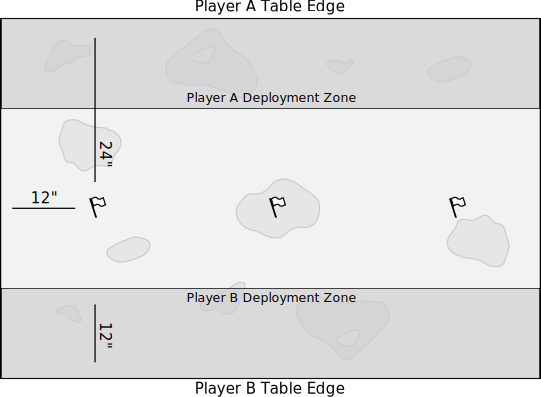
\includegraphics[scale=0.6]{maps/mission1}}

\missionheading{Mission 2: Forced March}

%\bigskip\centerline{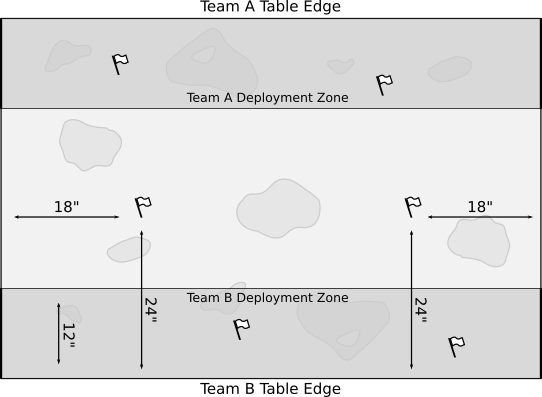
\includegraphics[scale=0.6]{maps/mission2}}

\missionheading{Mission 3: The Maelstrom}

\bigskip\centerline{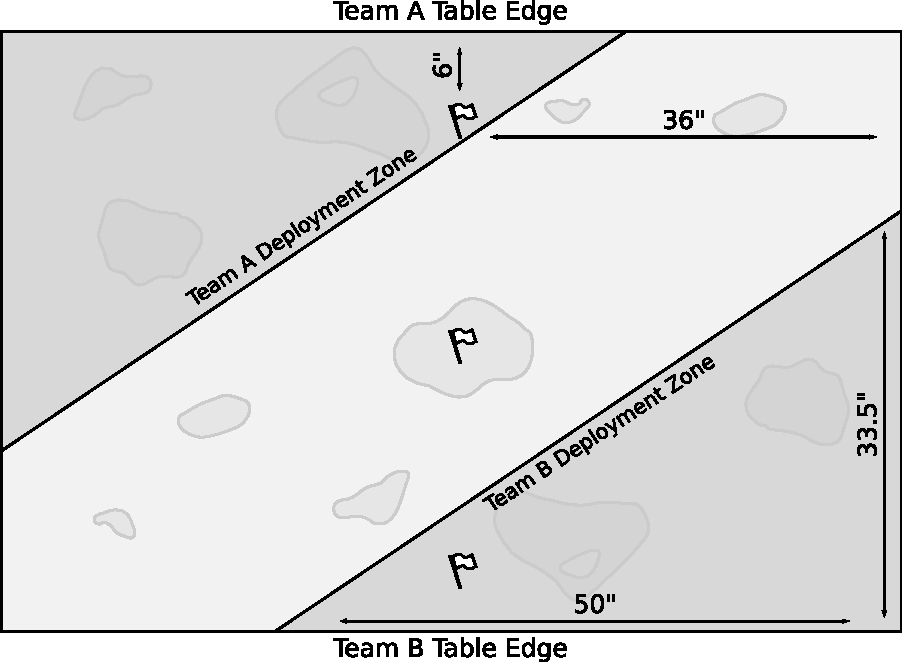
\includegraphics[scale=0.6]{maps/mission3}}


%%----------------------------------------------------------------------
%%----------------------------------------------------------------------
\clearpage
\missiontitle{Mission 1: Drop Zone}

\centerline{\emph{Rapid strike forces land and fight to carve out a
    beachhead for their armies.}}

\missionheading{Table Setup}

Deployment zones are the rectangles in each table corner~12'' in from
the long edge and~24'' in from the short edges.  The player that wins
the zone roll off picks either pair of \emph{diagonally opposite}
corners as their deployment zone and a long table edge as their player
edge.  The other player takes the other pair of diagonally opposite
corners and opposite long edge.

\bigskip%
After determining deployment zones, place five primary objective
markers: One at the center of the table worth~3 victory points; two
more 18'' from the short table edges and 24'' from the long table
edges worth~2 points each; and two~36'' from the short table edges and
12'' from the long table edges worth~1 point each.

\missionheading{Mission Specific Rules}

The following mission specific rules apply, in addition to those
applied to all missions in this pack.

\missionsubheading{Strike Force.}  All Fast Attack units have the
Obective Secured rule, as defined on page~122 of the rulebook.

%\missionsubheading{Nightfighting.}  All units have Stealth on Turn 1.



\missionheading{Scoring}

This mission is scored by objectives achieved, as follows.

\missionsubheading{Primary Objectives.}  Each primary objective marker
is worth their respective value given above.


\missionsubheading{Secondary Objectives.}

After deployment, both players simultaneously choose and then reveal a
single secondary objective for themselves from the list below.  Any
necessary selections are chosen and then revealed with the objective
unless noted otherwise.  \underline{No more than~6 victory points may
  be earned via any secondary.}

\begin{itemize}
\item \textit{Seize Ground.}  Choose two terrain pieces not in your
  deployment zone.  Do not declare these now, but do secretly record
  your selection unambiguously!  Reveal these at game end and score~3
  victory points for each piece that you control, treating them as
  objective markers.  Note that this means a single unit cannot claim
  both a primary objective marker and a terrain piece simultaneously.

\item \textit{Seek and Destroy.}  Choose and declare a Battlefield
  Role other than Troop.  Score~2 victory points for each enemy unit
  of this role completely destroyed or falling back at the end of the
  game.

\item \textit{Assassinate.}  Score~1 victory point for each opposing
  character model removed as a casualty or falling back at the end of
  the game.  Note that this is not limited to just independent
  characters.
\end{itemize}

\tertiaries


%%----------------------------------------------------------------------
%%----------------------------------------------------------------------
\clearpage
\missiontitle{Mission 2: Forced March}

\centerline{\emph{The armies begin the long maneuvers from their drop
    sites to the targets of their campaign.}}

\missionheading{Table Setup}

Deployment zones are \textbf{Hammer and Anvil}, as defined on page~131
of the main rulebook (24'' short edges).

\bigskip%
In each of the four table corners place a primary objective marker
12'' from both of the table edges of that corner.  Place a fifth
primary objective marker at the center of the table.

\missionheading{Mission Specific Rules}

The following mission specific rules apply, in addition to those
applied to all missions in this pack.

\missionsubheading{The Longest Day.}  After Turn~4 roll a D6; on a~4+
all units have Stealth for the remainder of the game.  Do this again
after Turn~5 if it did not take effect.  This rule automatically takes
effect after Turn~6.


\missionheading{Scoring}

This mission is scored by objectives achieved, as follows.

\missionsubheading{Primary Objectives.} At the conclusion of the game,
players score~1 victory point for each objective they control in their
own deployment zone and~2 points for the marker at table center.
Players earn~3 additional victory points if they control one marker in
the enemy deployment zone, and~5 points if they control both.

\missionsubheading{Secondary Objectives.}

After deployment, both players simultaneously choose and then reveal a
single secondary objective for themselves from the list below.  Any
necessary selections are chosen and then revealed with the objective
unless noted otherwise.  \underline{No more than~6 victory points may
  be earned via any secondary.}

\begin{itemize}
\item \textit{Control the Field.}  Each table quarter in which you
  have a scoring unit and your opponent does not, or you have an
  Objective Secured Unit and your opponent does not, is worth 2
  victory points.

\item \textit{Seek and Destroy.}  Choose and declare a Battlefield
  Role other than Troop.  Score~2 victory points for each enemy unit
  of this role completely destroyed or falling back at the end of the
  game.

\item \textit{Meatgrinder.}  Score~1 victory point for each opposing
  Troop unit destroyed or falling back at game end.

\end{itemize}

\tertiaries


%%----------------------------------------------------------------------
%%----------------------------------------------------------------------
\clearpage
\missiontitle{Mission 3: Into the Maelstrom}

\centerline{\emph{Now deep into the conflict, plans and strategies
    begin to fall apart.}}

\missionheading{Table Setup}

Deployment zones are \textbf{Vanguard Strike}, as defined on page~131
of the main \emph{Warhammer 40,000} rulebook.  Vanguard Strike may be
approximated by deploying within a 33.5'' x 50'' table corner
triangle.  The player that wins the zone roll off may pick any of the
four corners, and the other player takes that diagonally opposite.

\bigskip%
After determining deployment zones, roll off on~D6 and in that order
alternate placing objective markers.  Each player must place their
first marker in their opponent's deployment zone, their second in
neither zone, and their third in their own deployment zone.  Label
these markers~1 through~6, in any fashion.

\bigskip%
Both players receive their own table of tactical objectives, attached.


\missionheading{Mission Specific Rules}

At the start of each of your turns, do the following until you have 3
tactical objectives in play: Roll a~D3 and a~D6 and consult your
tactical objective table.  If that objective is already in play, has
been achieved, or is scratched off, roll both dice again.  Similarly,
if that objective would be provably impossible to accomplish in the
remainder of this game, e.g., your warlord has already been removed as
a casualty or your opponent has no characters remaining, roll both
dice again.  Once a valid objective has been rolled, mark it as in
play.

\smallskip%
At the end of each of your turns, check the requirement for each
tactical objective you have in play.  For each condition met, mark the
objective as achieved and score the associated value in \emph{tactical
  points} (n.b.: not \emph{victory points}).  Once achieved,
objectives are no longer considered in play and cannot be scored
again.  Multiple objectives can be scored in a turn, caveat that you
cannot score multiple tactical objectives with the same exact title in
the same turn using the same achievement.  E.g., to score both Storm
objectives at once, you would need to simultaneously control two
separate markers in the enemy deployment zone.

At the end of your you may also scratch out one of your tactical
objectives in play to remove it from play.

\smallskip
Tactical objectives in play, achieved, and scratched out are not secret.


\missionheading{Scoring}

This mission is scored by objectives achieved, as follows.

\missionsubheading{Primary Objectives.}

At game end, compare tactical points earned through tactical
objectives achieved and award victory points to the higher and lower
scorer as follows:

%\definecolor{Gray}{gray}{0.9}
%\definecolor{DGray}{gray}{0.75}
\newcolumntype{a}{>{\columncolor{gray!25}}c}
\newcolumntype{b}{>{\columncolor{gray!50}}r}
\bigskip\centerline{\setlength{\tabcolsep}{12pt}%
\begin{tabular}{|b|c|a|c|a|c|a|}
\hline
{\bf Difference}     & 0     & 1--2  & 3--4  & 5--6  & 7     & 8+\\
{\bf Victory Points} & 4 / 4 & 5 / 4 & 6 / 3 & 7 / 2 & 8 / 1 & 9 / 0\\
\hline
\end{tabular}}

% \begin{squishitemize}
%\item Difference of 0 Mission points = 4 - 4
%\item Difference of 1-2 MP = 5 - 4
%\item Difference of 3-4 MP = 6 - 3
%\item Difference of 5-6 MP = 7 - 2
%\item Difference of 7 MP = 8 - 1
%\item Difference of 8+ MP = 9 - 0
%\end{squishitemize}

\missionsubheading{Secondary Objectives.}

After deployment, both players simultaneously choose and then reveal a
single secondary objective for themselves from the list below.  Any
necessary selections are chosen and then revealed with the objective
unless noted otherwise.  \underline{No more than~6 victory points may
  be earned via any secondary.}

\begin{itemize}
\item \textit{Break Their Back.}  At game end, each enemy unit that
  has been eliminated, is falling back, or has at most~25\% of its
  starting models remaining is broken.  Earn~2 victory points per
  quartile if at least 25\%, 50\%, and 75\% of your opponent's army by
  units is broken.

\item \textit{Hold the Field.}  At game end, earn~2 victory points
  for every~2 primary objectives held.

\end{itemize}

\tertiaries

\clearpage

\newcounter{tonum}
\newcounter{tomajor}

\newcommand{\toblocktitle}{%
%\pagetitle{Primary Objectives}

\bigskip
\setcounter{tomajor}{1}%
\renewcommand{\arraystretch}{1.2}%
\noindent\hfill\begin{tabular}{F{2em}F{1em}F{1em}F{1em}F{1in}m{4.7in}}%4.7in
%\rowcolor{gray!50}
{\bf \#} & \hbox to 10pt{\hspace{-2pt}\rotatebox{45}{\bf In Play}}  & \hbox to 10pt{\hspace{-2pt}\rotatebox{45}{\bf Achieved}} & \hbox to 10pt{\hspace{-2pt}\rotatebox{45}{\bf Value}} & {\bf Title} & {\bf Requirement} \\
\end{tabular}\hfill\hbox to 0pt{}
}

\newenvironment{toblock}
{%
\setcounter{tonum}{1}
\rowcolors{1}{gray!25}{white}%
\renewcommand{\arraystretch}{1.2}%
\noindent\hfill\begin{tabular}{|C{2em}C{1em}C{1em}C{1em}C{1in}m{4.7in}|}
\hline
%\rowcolor{gray!50}
%{\bf \#} & \hbox to 10pt{\hspace{-2pt}\rotatebox{45}{\bf Drawn}}  & \hbox to 10pt{\hspace{-2pt}\rotatebox{45}{\bf Earned}} & \hbox to 10pt{\hspace{-2pt}\rotatebox{45}{\bf Points}} & {\bf Title} & {\bf Requirement} \\
%\hline
}
{%
\hline
\end{tabular}\hfill\hbox to 0pt{}
\stepcounter{tomajor}
}

\newcommand{\toset}{\setcounter{tonum}{1}\stepcounter{tomajor}}

\newcommand{\cardline}[3]{%
\thetomajor-\thetonum\stepcounter{tonum} & $\Box$ & $\Box$ & #3 & {\bf #1} & #2\\
}
% \raisebox{12pt}{\checkbox} & \raisebox{12pt}{\checkbox} 

\newcommand\tocard[3]{\cardline{#1}{#2}{#3}}
\WithSuffix\newcommand\tocard*[3]{\cardline{#1}{#2}{#3} [12pt]}

\newcommand{\totitle}[1]{%
\noindent\begin{tikzpicture}
\node [blackbox] (box){%
\vbox to 10pt {\vfil\hbox to \ttlwidth {\hfil%
\hbox {\color{white}\Large\bf\sc\fontfamily{ptm}\selectfont #1}
\hfil}\vfil%
}};%
\end{tikzpicture}%
%\vspace*{14pt}
}

%\totitle{Tactical Objectives}

%\begin{landscape}%
\squelchbackground%
%\resizebox{(\linewidth-3em)/2}{!}{%
%\begin{minipage}{(\linewidth-3em)/2}
\pagetitle{Player 1 Tactical Objectives}
\vfill
\clearpage
\squelchbackground
\begin{landscape}

\vspace*{-15pt}
\centerline{\scalebox{1.25}{\Large\bf\sc\fontfamily{ptm}\selectfont Tactical Objectives}}

\vspace{-24pt}
%\hrule
\vbox to 0pt{}

\noindent
\begin{minipage}[t][\textheight-0.25in][t]{0.5\linewidth-1em}
\resizebox{\linewidth}{!}{%
\begin{minipage}[t]{7.5in}%
\vbox to 0pt{}
\toblocktitle

\begin{toblock}
\tocard{Capture~1}{Control marker~\#1.}{1}
\tocard{Capture~2}{Control marker~\#2.}{1}
\tocard{Capture~3}{Control marker~\#3.}{1}
\tocard{Capture~4}{Control marker~\#4.}{1}
\tocard{Capture~5}{Control marker~\#5.}{1}
\tocard{Capture~6}{Control marker~\#6.}{1}
\end{toblock}

\bigskip
\begin{toblock}
\tocard{Capture~1}{Control marker~\#1.}{1}
\tocard{Capture~2}{Control marker~\#2.}{1}
\tocard{Capture~3}{Control marker~\#3.}{1}
\tocard{Capture~4}{Control marker~\#4.}{1}
\tocard{Capture~5}{Control marker~\#5.}{1}
\tocard{Capture~6}{Control marker~\#6.}{1}
\end{toblock}

\bigskip
\begin{toblock}
\tocard{Advance}{Control a marker outside both deployment zones.}{1}%
\tocard{Advance}{Control a marker outside both deployment zones.}{1}%
 \tocard{Storm}{Control a marker in your
  opponent's deployment zone.}{2}%
\tocard{Storm}{Control a marker in your opponent's deployment
  zone.}{2}%
\tocard{Defend}{Control all markers in your deployment zone; cannot
  score Turn 1.}{2}%
\tocard{Defend}{Control all markers in your deployment zone; cannot
  score Turn 1.}{2}%
\end{toblock}

\bigskip
\begin{toblock}
  \tocard{Take The Center}{Have a non-vehicle scoring unit wholly
    within~6'' of table center while your opponent has no scoring
    units even partially in the same.}{1}%
%
  \tocard{Stand The Wall}{At least 3 of your scoring units are
    within~12'' of your table edge and your opponent does not have any
    in the same; cannot score Turn 1.}{1}%
%
  \tocard{Breakthrough}{At least 2 of your scoring units are
    within~12'' of your opponent's table edge; cannot score Turn
    1.}{1}%
%
  \tocard{Secure The Perimeter}{Have a non-vehicle scoring unit in a
    table quarter in which your opponent does not have a scoring unit;
    cannot score Turn 1.}{2}%
%
  \tocard{Seize Momentum}{Control at least two more markers than your
    opponent.}{2}%
%
  \tocard{Clear A Path}{Control at least one marker in both deployment
    zones and at least one marker outside both.}{3}%
\end{toblock}
%
\end{minipage}}

\vfill
\small

Tactical objectives with a value of X may be kept in play as long as
you wish.  At the end of your any of your turns while in play they may
be marked as achieved and scored as indicated.

\smallskip%
Targets cannot be nominated or chosen for a tactical objective marked
with a $\dagger$ that have already been chosen for a $\dagger$
objective you have in play.

\smallskip%
Multiple tactical objectives with the exact same title cannot be
achieved at the same time using the same markers or opposing units.
\end{minipage}
\hfill
\begin{minipage}[t][\textheight-0.25in][t]{0.5\linewidth-1em}
\resizebox{\linewidth}{!}{%
\begin{minipage}[t]{7.5in}%
\vbox to 0pt{}
\toblocktitle*

\begin{toblock}
  \tocard{Frontfield \raisebox{6pt}{$\dagger$}}{When first put in
    play, choose a marker in your opponent's deployment zone.  At the
    end of your turns while in play, mark one of these boxes if you
    control that objective: \hfill $\Box$ $\Box$ $\Box$
    $\Box$\newline%
    \hbox to 0pt{}\hfill\emph{Value:} 1 mission point for each marked
    box.}{X}%
%
  \tocard{Midfield \raisebox{6pt}{$\dagger$}}{When first put in play,
    choose a marker in neither deployment zone.  At the end of your
    turns while in play, mark one of these boxes if you control that
    objective: \hfill $\Box$ $\Box$ $\Box$ $\Box$\newline%
    \hbox to 0pt{}\hfill\emph{Value:} 1 mission point for each marked
    box.}{X}%
%
  \tocard{Backfield \raisebox{6pt}{$\dagger$}}{When first put in play,
    choose a marker in your deployment zone.  At the end of your turns
    while in play, mark one of these boxes if you control that
    objective: \hfill $\Box$ $\Box$ $\Box$ $\Box$\newline%
    \hbox to 0pt{}\hfill\emph{Value:} 1 mission point for each marked
    box.}{X}%
%
%
  \tocard{Conqueror \raisebox{6pt}{$\dagger$}}{When first put in play,
    your opponent nominates two markers, of which you choose one.  At
    the end of your turns while in play, mark a box if you control
    that objective: \hfill $\Box$ $\Box$ $\Box$ $\Box$\newline%
    \hbox to 0pt{}\hfill\emph{Value:} 1 mission point for each marked
    box.}{X}%
%
  \tocard{Defender \raisebox{6pt}{$\dagger$}}{When first put in play,
    you nominate two markers, of which your opponent chooses one.  At
    the end of your turns while in play, mark a box if you control the
    chosen objective: \hfill $\Box$ $\Box$ $\Box$ $\Box$\newline%
    \hbox to 0pt{}\hfill\emph{Value:} 1 mission point for each marked
    box.}{X}%
%
  \tocard{Warrior}{When first put in play, your opponent nominates 3
    of their units.  Mark a box whenever one of those units is removed
    from play: \hfill $\Box$ $\Box$ $\Box$\newline%
    \hbox to 0pt{}\hfill\emph{Value:} 2 mission points for each
    marked box.}{X}%
\end{toblock}


\bigskip%
\begin{toblock}
  \tocard{Butcher}{While in play, mark one of these boxes each time an
    opposing non-vehicle, originally multi-model unit is removed from
    play: \hfill $\Box$ $\Box$ $\Box$ $\Box$\newline%
    \hbox to 0pt{}\hfill\emph{Value:} 1 mission point for each marked
    box.}{X}%
%
  \tocard{Hunter}{While in play, mark one of these boxes each time an
    opposing vehicle or monstrous creature is removed from play:
    \hfill $\Box$ $\Box$ $\Box$ $\Box$\newline%
    \hbox to 0pt{}\hfill\emph{Value:} 1 mission point for each marked
    box.}{X}%
%
  \tocard{Purifier}{While in play, mark one of these boxes each time
    an opposing unit with the Psyker, Psychic Pilot, or Brotherhood of
    Psykers/Sorcerers special rule is removed from play: \hfill $\Box$
    $\Box$ $\Box$ $\Box$\newline%
    \hbox to 0pt{}\hfill\emph{Value:} 1 mission point for each marked
    box.}{X}%
%
  \tocard{Assassin}{While in play, mark one of these boxes each time
    an opposing character is removed from play: \hfill $\Box$ $\Box$
    $\Box$ $\Box$\newline%
    \hbox to 0pt{}\hfill\emph{Value:} 1 mission point for each marked
    box.}{X}%
%
  \tocard{Harasser}{Contest or claim as many markers as possible;
    cannot score Turn 1.\newline%
    \hbox to 0pt{}\hfill\emph{Value:} 4 mission points minus
    the\newline \hbox to 0pt{}\hfill number of markers controlled by
    your opponent, to a minimum of 0.}{X}%
%
  \tocard{Commander}{Claim as many markers as possible; cannot score
    Turn 1.\newline%
    \hbox to 0pt{}\hfill\emph{Value:} 1 mission point for each marker
    you control.}{X}

\end{toblock}
%
\end{minipage}}

\vfill
\small

Immediately reroll any objectives provably impossible to achieve.

\smallskip%
No aspect of these tactical objectives is to be kept secret.
\end{minipage}

%\vfill
%\hrule
\end{landscape}

\clearpage
\restorebackground
%
\vfill\vbox to 0pt{}
%\end{minipage}%
%}%
%\hfill%
%\resizebox{(\linewidth-3em)/2}{!}{%
%\begin{minipage}{7.5in}%

\clearpage
\pagetitle{Player 2 Tactical Objectives}
\vfill
\clearpage
\squelchbackground
\begin{landscape}

\vspace*{-15pt}
\centerline{\scalebox{1.25}{\Large\bf\sc\fontfamily{ptm}\selectfont Tactical Objectives}}

\vspace{-24pt}
%\hrule
\vbox to 0pt{}

\noindent
\begin{minipage}[t][\textheight-0.25in][t]{0.5\linewidth-1em}
\resizebox{\linewidth}{!}{%
\begin{minipage}[t]{7.5in}%
\vbox to 0pt{}
\toblocktitle

\begin{toblock}
\tocard{Capture~1}{Control marker~\#1.}{1}
\tocard{Capture~2}{Control marker~\#2.}{1}
\tocard{Capture~3}{Control marker~\#3.}{1}
\tocard{Capture~4}{Control marker~\#4.}{1}
\tocard{Capture~5}{Control marker~\#5.}{1}
\tocard{Capture~6}{Control marker~\#6.}{1}
\end{toblock}

\bigskip
\begin{toblock}
\tocard{Capture~1}{Control marker~\#1.}{1}
\tocard{Capture~2}{Control marker~\#2.}{1}
\tocard{Capture~3}{Control marker~\#3.}{1}
\tocard{Capture~4}{Control marker~\#4.}{1}
\tocard{Capture~5}{Control marker~\#5.}{1}
\tocard{Capture~6}{Control marker~\#6.}{1}
\end{toblock}

\bigskip
\begin{toblock}
\tocard{Advance}{Control a marker outside both deployment zones.}{1}%
\tocard{Advance}{Control a marker outside both deployment zones.}{1}%
 \tocard{Storm}{Control a marker in your
  opponent's deployment zone.}{2}%
\tocard{Storm}{Control a marker in your opponent's deployment
  zone.}{2}%
\tocard{Defend}{Control all markers in your deployment zone; cannot
  score Turn 1.}{2}%
\tocard{Defend}{Control all markers in your deployment zone; cannot
  score Turn 1.}{2}%
\end{toblock}

\bigskip
\begin{toblock}
  \tocard{Take The Center}{Have a non-vehicle scoring unit wholly
    within~6'' of table center while your opponent has no scoring
    units even partially in the same.}{1}%
%
  \tocard{Stand The Wall}{At least 3 of your scoring units are
    within~12'' of your table edge and your opponent does not have any
    in the same; cannot score Turn 1.}{1}%
%
  \tocard{Breakthrough}{At least 2 of your scoring units are
    within~12'' of your opponent's table edge; cannot score Turn
    1.}{1}%
%
  \tocard{Secure The Perimeter}{Have a non-vehicle scoring unit in a
    table quarter in which your opponent does not have a scoring unit;
    cannot score Turn 1.}{2}%
%
  \tocard{Seize Momentum}{Control at least two more markers than your
    opponent.}{2}%
%
  \tocard{Clear A Path}{Control at least one marker in both deployment
    zones and at least one marker outside both.}{3}%
\end{toblock}
%
\end{minipage}}

\vfill
\small

Tactical objectives with a value of X may be kept in play as long as
you wish.  At the end of your any of your turns while in play they may
be marked as achieved and scored as indicated.

\smallskip%
Targets cannot be nominated or chosen for a tactical objective marked
with a $\dagger$ that have already been chosen for a $\dagger$
objective you have in play.

\smallskip%
Multiple tactical objectives with the exact same title cannot be
achieved at the same time using the same markers or opposing units.
\end{minipage}
\hfill
\begin{minipage}[t][\textheight-0.25in][t]{0.5\linewidth-1em}
\resizebox{\linewidth}{!}{%
\begin{minipage}[t]{7.5in}%
\vbox to 0pt{}
\toblocktitle*

\begin{toblock}
  \tocard{Frontfield \raisebox{6pt}{$\dagger$}}{When first put in
    play, choose a marker in your opponent's deployment zone.  At the
    end of your turns while in play, mark one of these boxes if you
    control that objective: \hfill $\Box$ $\Box$ $\Box$
    $\Box$\newline%
    \hbox to 0pt{}\hfill\emph{Value:} 1 mission point for each marked
    box.}{X}%
%
  \tocard{Midfield \raisebox{6pt}{$\dagger$}}{When first put in play,
    choose a marker in neither deployment zone.  At the end of your
    turns while in play, mark one of these boxes if you control that
    objective: \hfill $\Box$ $\Box$ $\Box$ $\Box$\newline%
    \hbox to 0pt{}\hfill\emph{Value:} 1 mission point for each marked
    box.}{X}%
%
  \tocard{Backfield \raisebox{6pt}{$\dagger$}}{When first put in play,
    choose a marker in your deployment zone.  At the end of your turns
    while in play, mark one of these boxes if you control that
    objective: \hfill $\Box$ $\Box$ $\Box$ $\Box$\newline%
    \hbox to 0pt{}\hfill\emph{Value:} 1 mission point for each marked
    box.}{X}%
%
%
  \tocard{Conqueror \raisebox{6pt}{$\dagger$}}{When first put in play,
    your opponent nominates two markers, of which you choose one.  At
    the end of your turns while in play, mark a box if you control
    that objective: \hfill $\Box$ $\Box$ $\Box$ $\Box$\newline%
    \hbox to 0pt{}\hfill\emph{Value:} 1 mission point for each marked
    box.}{X}%
%
  \tocard{Defender \raisebox{6pt}{$\dagger$}}{When first put in play,
    you nominate two markers, of which your opponent chooses one.  At
    the end of your turns while in play, mark a box if you control the
    chosen objective: \hfill $\Box$ $\Box$ $\Box$ $\Box$\newline%
    \hbox to 0pt{}\hfill\emph{Value:} 1 mission point for each marked
    box.}{X}%
%
  \tocard{Warrior}{When first put in play, your opponent nominates 3
    of their units.  Mark a box whenever one of those units is removed
    from play: \hfill $\Box$ $\Box$ $\Box$\newline%
    \hbox to 0pt{}\hfill\emph{Value:} 2 mission points for each
    marked box.}{X}%
\end{toblock}


\bigskip%
\begin{toblock}
  \tocard{Butcher}{While in play, mark one of these boxes each time an
    opposing non-vehicle, originally multi-model unit is removed from
    play: \hfill $\Box$ $\Box$ $\Box$ $\Box$\newline%
    \hbox to 0pt{}\hfill\emph{Value:} 1 mission point for each marked
    box.}{X}%
%
  \tocard{Hunter}{While in play, mark one of these boxes each time an
    opposing vehicle or monstrous creature is removed from play:
    \hfill $\Box$ $\Box$ $\Box$ $\Box$\newline%
    \hbox to 0pt{}\hfill\emph{Value:} 1 mission point for each marked
    box.}{X}%
%
  \tocard{Purifier}{While in play, mark one of these boxes each time
    an opposing unit with the Psyker, Psychic Pilot, or Brotherhood of
    Psykers/Sorcerers special rule is removed from play: \hfill $\Box$
    $\Box$ $\Box$ $\Box$\newline%
    \hbox to 0pt{}\hfill\emph{Value:} 1 mission point for each marked
    box.}{X}%
%
  \tocard{Assassin}{While in play, mark one of these boxes each time
    an opposing character is removed from play: \hfill $\Box$ $\Box$
    $\Box$ $\Box$\newline%
    \hbox to 0pt{}\hfill\emph{Value:} 1 mission point for each marked
    box.}{X}%
%
  \tocard{Harasser}{Contest or claim as many markers as possible;
    cannot score Turn 1.\newline%
    \hbox to 0pt{}\hfill\emph{Value:} 4 mission points minus
    the\newline \hbox to 0pt{}\hfill number of markers controlled by
    your opponent, to a minimum of 0.}{X}%
%
  \tocard{Commander}{Claim as many markers as possible; cannot score
    Turn 1.\newline%
    \hbox to 0pt{}\hfill\emph{Value:} 1 mission point for each marker
    you control.}{X}

\end{toblock}
%
\end{minipage}}

\vfill
\small

Immediately reroll any objectives provably impossible to achieve.

\smallskip%
No aspect of these tactical objectives is to be kept secret.
\end{minipage}

%\vfill
%\hrule
\end{landscape}

\clearpage
\restorebackground
%
\vfill\vbox to 0pt{}
%\end{minipage}%
%}%
%\end{landscape}

\clearpage
\restorebackground

\end{document}
